\documentclass{article}

% Language setting
% Replace `english' with e.g. `spanish' to change the document language
\usepackage[english]{babel}

% Set page size and margins
% Replace `letterpaper' with `a4paper' for UK/EU standard size
\usepackage[letterpaper,top=2cm,bottom=2cm,left=3cm,right=3cm,marginparwidth=1.75cm]{geometry}
\usepackage[backend=biber,style=numeric,sorting=ynt]{biblatex}

% Useful packages
\usepackage{amsmath}
\usepackage{graphicx}
\usepackage{multirow}
\usepackage[colorlinks=true, allcolors=blue]{hyperref}
\usepackage[table,xcdraw]{xcolor}

\addbibresource{bibliography.bib}
\title{ADM: Algorithms for Data Mining \\[1ex] \large An exploration of ensemble learning: AdaBoost vs XGBoost}
\author{Marc Maynou Yélamos }

\begin{document}
\maketitle

\begin{abstract}
Ensemble methods are becoming increasingly popular due to the generalize improvement that has been observed in the predictions generated with this methodology, becoming a real alternative to single, highly-complex models. This paper aims at exploring what ensemble methods are, describe its main types and elaborate a comparison between two of the most common methods: AdaBoost and XGBoost. Both conceptual and practical aspects of both algorithms will be explored, stating the main differences between its implementation alongside a practical execution of the systems to elaborate predictions.

\end{abstract}

\section{Ensemble methodology}
\subsection{Intuition behind the ensemble methodology}

When trying to choose a model to accurately predict future data, one might be tempted to default to the single, most-complex method available. It would make sense to rely on the algorithm that draws the best relationships among data and that is able to extract as many nuances as possible. However, another, equally valid approach is to take into account the \textbf{results of several predictors}, extracting a final conclusion from \textbf{combining the outputs of all of them}. Further down in the document we will explore why this second methodology is reasonable with data-related arguments, oftentimes yielding even better results than the usage of a single method. However, a more high-level explanation can also be given first as to introduce the intuitive utility of the ensemble methodology.

In our daily lives we use “ensemble methods” all the time, understanding by this the combination of different outputs to reach a conclusion or decision regarding a certain issue. For instance, we might read several reviews of a product before buying it, we might ask the opinions of several people before making our mind around a certain topic and we might even try to infer how an event is going to unfold (a party, a conversation, an exam, etc.) based on previous iterations. The primary goal is to prevent (or at least minimize) the probability of making the wrong decision. This is achieved through taking into consideration multiple sources of information and structuring our opinion around it, contrary to just consulting a single source and hoping it was correct.

However, as much as the aforementioned intuition makes sense, establishing a comparison between daily life and machine learning is not fair. This approach works in day-to-day issues as most of the time we have little to no information about the decision that we have to make and about which sources to consult. This means that by expanding our reference points, we avoid making a terrible decision. Data, on the other hand, is more concise, the problem to solve is more tightly bound and we tend to have a more precise body of knowledge to work with. This means that, even though ensemble methods have become considerably more popular given the generalized increase in accuracy that they provide, they should be taken into consideration as another tool to be used when needed. As with every machine learning problem, a careful study of the data, the goal and the methodology should be performed to select the best approach.

\subsection{Advantages of ensemble methods}
As stated before, the ensemble methodology makes intuitive sense. However, there are some other, more specific arguments that support its usage \textbf{\cite{Polikar:2009}}. The primary reason to do so is probably associated with answering one of the hardest questions in any machine learning project: which is the most appropriate predictor to use? Different algorithms may behave better in different scenarios, and to the initial complexity of this issue, we have to add the many parameters that have to be tuned for each one of them, which can considerably vary the performance. Even if we chose the predictor that performs best, we could just be relying on the accuracy scores obtained in the training data and the small amount of test data that is available, which can introduce a high variance in the model even when applying cross-validation. Combining different predictors does not always guarantee a better accuracy, but it certainly \textbf{reduces the probability of selecting a poor-performing single predictor}.

Another advantage of ensemble methods is its \textbf{flexibility}. With single predictors, too much or too little data might be an issue, given that it might have to spend too much time computing the predictions or not have enough data to create a generalized decision. Ensemble methods can deal with both of these issues. A dataset that is too large can be divided into different, smaller subsets that can be ingested by different predictors and its outcomes combined. On the other hand, with a dataset that is too small, bootstrapping techniques can be applied, drawing data with replacement and treating it as if it was independently drawn from the distribution.

The quantity of data already poses a big issue to the predictors, but \textbf{the problem that is trying to be solved} can also be an obstacle difficult to overcome. Some problems are just too difficult to tackle “on one go” or with one method, and that’s why divide and conquer techniques have been a popular method in algorithmics for a long time. These techniques consist of breaking down a problem into smaller subproblems to be tackled individually. This same pattern can be applied to machine learning when using a single predictor is a too rigid approach, and employing several, smaller and more specific predictors can make reaching a conclusion more feasible.

Lastly, the very structure of an ensemble system naturally\textbf{ assigns a confidence to each decision}. In most ensemble methods, the decision that is taken is the one that has appeared the most times, without considering if the difference regarding the other results is significant or not. For instance, if we use 99 predictors to solve a binary classification problem and, for a given instance, 50 of them predict label a, it will be assigned as the result. However, 49 of the predictors reached a different conclusion. This means that the confidence on the prediction is fairly low and, as such, it should be acknowledged that there is a high chance of it being incorrect. It is important to remark that a decision that has low confidence is not necessarily wrong and, conversely, high confidence does not guarantee correctness. However, it has been shown that there is a positive correlation between the confidence of a prediction and the probability of it being correct.

\subsection{Types of ensemble learning}

As it has been stated, ensemble learning consists of the usage of several, small predictors to solve a certain problem, rather than using a single, bigger and complex learner. However, there are different ways to do so. The main three ones are highlighted next:

\textbf{Bagging \cite{IBM}} (Bootstrap aggregating): this first technique combines the two methods its name is made of. First, a random sample of data is selected with replacement (i.e. the individual points can be selected multiple times, hence the bootstrap). Afterwards, the learners are trained independently using the data, and their results are aggregated to build the model. More specifically, if it is a classification problem, the option that appears most times for each data row is chosen, whereas for a regression problem the average value is selected instead. It is commonly used with learners that have high variance and low bias, as by using multiple learners we can more easily control the variance displayed by them. 

\textbf{Boosting \cite{IBM}}: boosting is very similar to bagging but with a crucial difference, which is that the learners are trained sequentially, trying to “fix” the issues that the previous learner had. This means that with each new iteration the misclassified data is made more relevant as to fix the weaknesses that appear in the learning process. An additional difference with regards to bagging is that boosting is usually applied with learners that have high bias and low variance. This is because of the fact that we are now taking into account the mistakes of the previous learner, allowing us to solve the intrinsic deviations that the learners make.

\textbf{Stacking \cite{Vidhya}}: stacking 3 applies a different procedure to that of both boosting and bagging. The first difference is that it uses different types of base learners, whereas the other two methods use different instatiations of the same type of learner. The main purpose of this approach is to benefit from applying different algorithms to a problem, each one solving the part of the issue it is best prepared to tackle. To do so, the learners are trained by a meta-learner that gathers the predictions and presents a final decision, learning the best way to combine the inputs to issue the most accurate prediction.

Once the three main types of ensemble algorithms have been presented, we will dive deeper into the two main algorithms that will be compared in this document: AdaBoost and XGBoost, both of which, as it can be guessed, belong to the boosting type.


\section{AdaBoost and XGBoost}

As stated in the introduction, the practical aspect of this report will include the comparison of two of the most used ensemble methods: AdaBoost and XGBoost. Before we present the results of the tests, it is important to understand the mechanisms behind both systems.

\subsection{Adaptive Boosting (AdaBoost)}

The base learners used in ensemble methods are also referred to as weak learners. In the context of regression, weak means that it is able to approximate the true value within a reasonable threshold, but still very far from the desired outcome. As for classification problems, the idea of a weak learner is more clearly seen, as it represents everything that can predict a class better than random guessing, but still performs poorly when trying to assign multiple classes. 

This is because they are based on very general patterns that work for a lot of cases but are not nuanced enough. For instance, we could guess that all people above 50 do not practice any kind of sport. You might get a high accuracy, but there are still a lot of misclassified points that, with some more variables and more developed patterns, could be correctly labeled. To better illustrate the rest of the AdaBoost explanation we will assume a classification problem.

Understanding what a weak learner represents is relevant, as AdaBoost \textbf{\cite{Vidhya2}}, \textbf{\cite{youtube}} tends to use one of the most simple learners: a decision stump. This is, essentially, the first level of a decision tree, with a single node, two leaves and a single criteria to classify the data (similar to the example presented above). A decision stump is not a good method to make decisions, especially compared to its fully developed variant, which uses more variables to make the predictions. However, \textbf{it is really fast to create and train}, two characteristics that are exploited by the boosting approach.

As stated beforehand, the boosting methodology relies on iteratively improving the predictions of the learners by taking into account the wrongly classified data of the previous learner. In the case of AdaBoost this is done by \textbf{assigning weights to each data point}, and modifying the weights accordingly with each iteration (i.e. data points mislabelled  when evaluating learner \textit{n} will have its weight increased when building learner \textit{n+1}. Consequently, correctly classified data has its weight reduced). This means that each new learner will prioritize \textbf{getting right the data points that the previous instantiation got wrong}, trying to improve the overall accuracy. This process of correcting mistakes is repeated for a given number of iterations, which has to be tuned.

As it can be deduced, correcting some misclassifications may imply that some data points that were correctly labeled will now have the wrong class assigned. This makes sense, given that we are working with decision stumps that only have a single variable to create a division. Therefore, by trying to fix the misclassified data, a different variable may be chosen with regard to the one used in the previous learner and, even though the goal of correcting the mistakes might be achieved, the overall accuracy might decrease as the new variable might be worse to deal with all the data points. If that is the case, trying to get those points right might not be beneficial as the overall performance is deteriorated.

In order to correct this issue, AdaBoost includes another mechanism: each individual learner (i.e. each individual stump) has a different weight in the final decision, meaning that the prediction of some stumps is \textbf{taken into more consideration than others}. This value is influenced by how accurate the predictions are. When a stump is trained and evaluated, the weights of the misclassified data points are added and introduced into the following formula inside the \textit{TotalError} variable:

\[\frac{1}{2} log \frac{1 - TotalError}{TotalError}\]

\begin{figure}
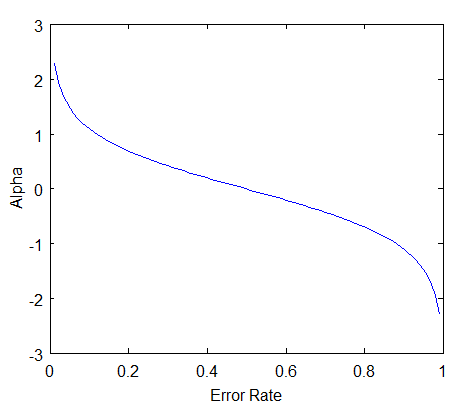
\includegraphics[scale=0.6]{plot.png}
\centering
\end{figure}

What is interesting about the results is that the importance of a stump increases exponentially as the error rate is reduced, making really good predictors way more relevant for the final classification than good, average or, logically, bad predictors. Additionally, the result of the function can be negative, which implies that the division a stump made can be negatively correlated with the true values. If that is the case, the importance of the stump is also high, but in an inverse way.

\subsection{Extreme Gradient Boosting (XGBoost)}

XGBoost is a more sophisticated version of another boosting algorithm: gradient boosting (eXtreme Gradient Boosting). Therefore, in order to fully comprehend XGBoost, it is necessary to first overview the main characteristics of gradient boosting.

Gradient boosting \textbf{\cite{Vidhya3}}, \textbf{\cite{youtube2}} follows a very similar structure as AdaBoost, building a model based on a lot of weak learners that compensate for the mistakes of previous learners. However, there’s some crucial difference between both methods. The first one is that gradient boosting usually does \textbf{not limit the size of the trees to one level} (stump), but instead builds bigger trees (although they are still limited to four or five intermediate nodes). Additionally, whereas AdaBoost scaled the contribution of each tree based on the accuracy of the predictions, Gradient Descent scales all the trees by the same value.

To go over Gradient Boosting, we will use a regression problem. The first step is to generate a single leaf that will act as the initial prediction. In the case of regression, this is as simple as taking the average value of the target variable. The next step is to build a tree based on the errors of this first naive prediction. What is meant by error is, in this case, the difference between the real value (observed value) and our prediction (predicted value). This will generate so-called pseudo residuals, a term that gradient boosting adopts from linear regression. Therefore, the new tree will \textbf{try to predict the residuals, not the observed value}. This may sound counter-intuitive, but Gradient Boosting does function in this way because it is trying to, at each step, reduce the difference between the prediction and the observed value through reducing the value of the residual. This will be further explained in the next paragraphs.

Once the new tree is built, we will run the data through it, adding the predicted pseudo residual to the initial value that we had (the average). This will yield results that are closer to the real values than just taking the average into account. However, we may notice that the predictions fit the training data too well. This is not desirable as we may be introducing a lot of variance into the model, which implies that it will perform poorly on unseen data. To solve this problem, Gradient Boosting introduces a \textbf{learning rate to scale the contribution of the tree}.

Even though the learning rate can be any value between 0 and 1, in practice it tends to take value closer to 0 (i.e. 0.1, 0.2). This is due to the “gradient” algorithmic approach of taking a lot of smaller steps towards the right direction, which reduces the potential variance at the expense of some bias. As stated above, the learning rate is the same for all trees.

Once the first tree is built the process will iteratively continue, building new trees that try to predict the pseudo residuals that are obtained from the difference of the observed value and the value predicted by the previous tree (which is based on the predictions of all the trees before it, hence the boosting aspect to it). For instance, after the second tree is built, the new predicted value will be the average (initial prediction) plus the predicted residual of the first tree and the predicted residual of the second tree (both scaled by the learning rate).

Ideally, the new predicted value will be closer to the observed value. However, at each new step the distance will be reduced in a lesser amount, meaning that at each iteration the “steps” will be smaller. This is so because the residuals will get smaller every time and so the potential reduction is also smaller. Gradient Boosting will keep generating trees until it reaches a maximum specified or the addition of new trees does not significantly reduce the size of the residuals (i.e. they have converged). If instead of a regression problem we have to deal with a classification problem, the process is very similar, with the main difference that it will use the logarithm of the odds (\textit{log(odds))} to compute the distances.

As stated at the beginning of the section, XGBoost \textbf{\cite{datascience}}, \textbf{\cite{youtube3}} is a complex machine learning algorithm that combines a lot of parts and optimizations to make the gradient boosting process better and faster. The main change is the usage of a unique kind of trees, that are built through the calculation of \textit{similarity scores} and \textit{gain} to split the data, and pruned through a complexity parameter. This distinct way of building the trees allows XGBoost to present better accuracy scores than most other algorithms for generalized scenarios. However, it also includes computational improvements such as parallel learning, cache-awareness access or approximate greedy algorithms.

\section{Practical comparison}
On paper, XGBoost should be a more complete method, providing better results in less time. This is because XGBoost was developed with these goals in mind, hence the optimization presented beforehand. This should be specially true for large dataset, in which the improvements should be more noticeable. AdaBoost, even though it is relatively robust to overfitting in low noise datasets, when there is a lot of noise data may yield considerably worse results, given that it might spend too much time learning extreme cases and skewing the results. Moreover, it was not designed with efficiency in mind. On paper, the only downside to XGBoost is the existence of a lot of hyperparameters than need to be tuned, which might make it hard to get the best results possible out of it. This, however, should not be a big issue given that the standard configuration provides great results for a vast majority of scenarios.
\subsection{Data and experimental procedure}

In order to put to the test the theoretical differences between AdaBoost and XGBoost, I decided to compare them in a practical environment. More specifically, 5 different tests were performed, which involved the generation of predictions over 4 different datasets. The main purpose was to see the differences in the performance of both algorithms and check whether the upgrades of XGBoost did impact the performance. As for the tests, both XGBoost and AdaBoost are suited to deal with classification as well as regression problems. So, in order to realize a more thorough comparison, three of the tests will perform classification tasks and two tests will perform regression tasks. The five tests will be performed over four different datasets:

\begin{itemize}
    \item \textit{Iris} dataset \footnote{https://archive.ics.uci.edu/ml/datasets/iris} (classification): it classifies iris plants into three different categories based on various dimensions of the plants. It presents 5 columns, a lower cardinality (150 instances) and three possible labels for the target.
    \item \textit{Mushrooms} dataset \footnote{https://www.kaggle.com/datasets/uciml/mushroom-classification} (classification): includes descriptions of mushroom species for 2 big families. As a result, this dataset is suited for a binary classification problem in which we try to predict to which family a given mushroom belongs. There are 21 columns and over 9.100 instances.
    \item \textit{Diamonds} dataset \footnote{https://www.kaggle.com/datasets/shivam2503/diamonds} (classification and regression): this dataset presents information about prices, weights and other attributes of diamonds. A lot of the variables could be chosen to perform prediction of, which is a very unique characteristic of the dataset. From a total of 11 columns, two will be chosen as the targets: the cut (i.e. the quality of the diamond, 5 possible labels) for classification and the price for regression. This dataset also contains a lot of data, with almost 54.000 instances.
    \item \textit{KC house} dataset \footnote{https://www.kaggle.com/datasets/shivachandel/kc-house-data} (regression): this dataset gathers a lot of information regarding houses in King County, Washington. The goal is to try to predict the price of the house based on the properties it presents. There are 20 different variables and over 26.000 instances.
\end{itemize}

As it can be observed, the datasets are quite varied, not only in the tasks they will be used for (binary and multiclass classification and regression) but also in its size, quantity of predictors and type of the columns. The goal was to generate different scenarios so the differences could be seen more clearly.

It is also important to consider that AdaBoost and XGBoost can have different configurations to modify how its execution is performed. As the goal of the experiment is to compare its efficiency (and not getting the best accuracy), the parameters used are going to be the default ones. However, both algorithms are based on smaller algorithms to perform the boosting with. Different algorithms can perform vastly differently depending on the dataset, so I decided to, for each test, try different base learners, all of them of a relatively low complexity. More specifically:

\begin{itemize}
    \item AdaBoost: it is important to mention that in the explanation of the algorithm I used the stumps as weak learners because it was the most comprenhensible way to diaply the features of the method. However, AdaBoost can use a variety of base learners that, if used properly, tend to yield better results while also maintaning the complexity of the algorithm low. Using a variety of these algorithms makes for a more interesting comparison than just using stumps. As such, the next weak learner will be used for classification: decision trees (not limited to one level), ridge classification, multinomial naive bayes and perceptron. As for regression, decision trees, linear regression, RANSAC algorithm and bayesian ridge will be used. 

    \item XGBoost: differently form gradient boosting, XGBoost is more limited in the learners that it implemenets, as they are all based on the unique way of building trees that it presents. The documentation of the XGBoost library for python indicates that there are three different methods available: gbtree, dart and gblinear. The first two correspond to tree based models, while the last one is based on linear functions. All of them will be used in the evaluation of each dataset.
\end{itemize}
\subsection{Results and conclusions}

The code was developed using python notebooks with libraries such as pandas, scikit-learn, numpy or feature-engine for the implementation of the methods. The code can be found in the next address: \url{https://github.com/marc-maynou/ADM-Deliverable-2/tree/main/Code}. The results of the experiments are illustrated in tables 1 and 2. In each, we can observe the metric obtained for all the datasets involved. These results are also separated by the learner used when executing each algorithm.

The first conclusion that can be reached is quite evident: XGBoost performs best than AdaBoost acros the board. Not taking into account the GBLinear learner and using the standard tree approach, XGBoost always performs better. This is specially noticeable for the bigger and more complex datasets (\textit{diamond} for classification and \textit{KC House} for regression), where XGBoost is considerably better than AdaBoost for all its configurations. As stated, this make sense, given that XGBoost was designed to tackle harder datasets.

In the classification tasks, AdaBoost performs best with decision trees, which come considerably close to the accuracy obtained by XGBoost. However, for regression tasks, the other three methods perform, on average, better. This implies that the precision of the predictions can vary considerable depending on the algorithm use. This presents yet another issue with AdaBoost, which is that we do not know which learner might be the best performer. We might have some clues based on the kind of problem that it is being faced, but an exploration of several methods might be necessary. On the contrary, XGBoost presents only two main learners that, as can be seen, perform exactly the same (at least for the data used). This, as mentioned in previous sections, comes with the detriment of incorporating a lot of configuration parameters. However, it can also be seen that the base parametrization yields noticeably good results, so it might not be necessary to alter the values in a the vast majority of situations.

In terms of execution time, I did not appreciate any major difference between AdaBoost and XGBoost. Maybe the size of the data was not big enough (or the number of iterations not high enough) for any differentiation to be visible. Altering the base configuration of both systems to generate longer executions might evidence the improvements of XGBoost in terms of time consumption.

Summarizing the results,we can see that AdaBoost is a good approach when dealing with datasets of a moderate complexity, specially compared with other techniques. However, in terms of performance, XGBoost is always superior, even for the smaller dataset, which makes it an almost-always better tool to use. This statement, which is confirmed in the boundaries of this experiment, is also backed up by the current literature and practises, as XGBoost is used in a considerably bigger amount than AdaBoost. Logically, to create further evidence for this, it would be necessary to elaborate more tests, over more datasets, with more configurations and with a more developed preprocessing/evaluation. However, within the limited confines of these trials, the theoretically better performance of XGBoost has been clearly presented. Personally, the exploration of the ensemble methodologies as well as both AdaBoost and XGBoost has been very interesting, as they were topics that I has not treated previously, and they have surely become a tool that I will have very present when facing other machine learning tasks.


\begin{table}[]
\begin{tabular}{|ccccc}
\hline
\rowcolor[HTML]{333333} 
\multicolumn{5}{|c|}{\cellcolor[HTML]{333333}{\color[HTML]{FFFFFF} Accuracy in the classification tasks (\%)}}                                                                                                                                                                                                                                                                                                                         \\ \hline
\rowcolor[HTML]{656565} 
\multicolumn{2}{|c|}{\cellcolor[HTML]{656565}}                                                                                                                  & \multicolumn{1}{c|}{\cellcolor[HTML]{656565}{\color[HTML]{FFFFFF} Iris dataset}} & \multicolumn{1}{c|}{\cellcolor[HTML]{656565}{\color[HTML]{FFFFFF} Mushroom dataset}} & \multicolumn{1}{c|}{\cellcolor[HTML]{656565}{\color[HTML]{FFFFFF} Diamonds dataset (cut)}} \\ \hline
\multicolumn{1}{|c|}{\cellcolor[HTML]{656565}{\color[HTML]{FFFFFF} }}                           & \multicolumn{1}{c|}{\cellcolor[HTML]{C0C0C0}Decision Trees}   & 91.11                                                                            & 100                                                                                  & 68.12                                                                                      \\ \cline{2-2}
\rowcolor[HTML]{EFEFEF} 
\multicolumn{1}{|c|}{\cellcolor[HTML]{656565}{\color[HTML]{FFFFFF} }}                           & \multicolumn{1}{c|}{\cellcolor[HTML]{C0C0C0}Ridge classifier} & 88.89                                                                            & 100                                                                                  & 51.96                                                                                      \\ \cline{2-2}
\multicolumn{1}{|c|}{\cellcolor[HTML]{656565}{\color[HTML]{FFFFFF} }}                           & \multicolumn{1}{c|}{\cellcolor[HTML]{C0C0C0}Naive Bayes}      & 77.78                                                                            & 97.74                                                                                & 20.57                                                                                      \\ \cline{2-2}
\rowcolor[HTML]{EFEFEF} 
\multicolumn{1}{|c|}{\multirow{-4}{*}{\cellcolor[HTML]{656565}{\color[HTML]{FFFFFF} AdaBoost}}} & \multicolumn{1}{c|}{\cellcolor[HTML]{C0C0C0}Perceptron}       & 93.33                                                                            & 100                                                                                  & 39.70                                                                                      \\ \hline
\multicolumn{1}{|c|}{\cellcolor[HTML]{656565}{\color[HTML]{FFFFFF} }}                           & \multicolumn{1}{c|}{\cellcolor[HTML]{C0C0C0}GBTree}           & 97.77                                                                            & 100                                                                                  & 74.40                                                                                      \\ \cline{2-2}
\rowcolor[HTML]{EFEFEF} 
\multicolumn{1}{|c|}{\cellcolor[HTML]{656565}{\color[HTML]{FFFFFF} }}                           & \multicolumn{1}{c|}{\cellcolor[HTML]{C0C0C0}Dart}             & {\color[HTML]{333333} 97.77}                                                     & {\color[HTML]{333333} 100}                                                           & {\color[HTML]{333333} 74.40}                                                               \\ \cline{2-2}
\multicolumn{1}{|c|}{\multirow{-3}{*}{\cellcolor[HTML]{656565}{\color[HTML]{FFFFFF} XGBoost}}}  & \multicolumn{1}{c|}{\cellcolor[HTML]{C0C0C0}GBlinear}         & 60.00                                                                            & 89.66                                                                                & 40.05                                                                                      \\ \cline{1-2}
\end{tabular}
\centering
\caption{Accuracy obtained in the development of the classification tests}
\end{table}

\begin{table}[]
\begin{tabular}{cccc}
\hline
\rowcolor[HTML]{333333} 
\multicolumn{4}{c}{\cellcolor[HTML]{333333}{\color[HTML]{FFFFFF} R-squared obtained in the regression tasks (\%)}} \\ \hline
\rowcolor[HTML]{656565} 
\multicolumn{2}{|c|}{\cellcolor[HTML]{656565}} &
  \multicolumn{1}{c|}{\cellcolor[HTML]{656565}{\color[HTML]{FFFFFF} Diamond dataset (price)}} &
  \multicolumn{1}{c|}{\cellcolor[HTML]{656565}{\color[HTML]{FFFFFF} KC House dataset}} \\ \hline
\multicolumn{1}{|c|}{\cellcolor[HTML]{656565}{\color[HTML]{FFFFFF} }} &
  \multicolumn{1}{c|}{\cellcolor[HTML]{C0C0C0}Decision Trees} &
  86.70 &
  \multicolumn{1}{c|}{36.45} \\ \cline{2-2}
\rowcolor[HTML]{EFEFEF} 
\multicolumn{1}{|c|}{\cellcolor[HTML]{656565}{\color[HTML]{FFFFFF} }} &
  \multicolumn{1}{c|}{\cellcolor[HTML]{C0C0C0}Linear regression} &
  88.76 &
  \multicolumn{1}{c|}{\cellcolor[HTML]{EFEFEF}49.70} \\ \cline{2-2}
\multicolumn{1}{|c|}{\cellcolor[HTML]{656565}{\color[HTML]{FFFFFF} }} &
  \multicolumn{1}{c|}{\cellcolor[HTML]{C0C0C0}RANSAC} &
  86.86 &
  \multicolumn{1}{c|}{46.78} \\ \cline{2-2}
\rowcolor[HTML]{EFEFEF} 
\multicolumn{1}{|c|}{\multirow{-4}{*}{\cellcolor[HTML]{656565}{\color[HTML]{FFFFFF} AdaBoost}}} &
  \multicolumn{1}{c|}{\cellcolor[HTML]{C0C0C0}Bayesian Ridge} &
  88.54 &
  \multicolumn{1}{c|}{\cellcolor[HTML]{EFEFEF}49.83} \\ \hline
\multicolumn{1}{|c|}{\cellcolor[HTML]{656565}{\color[HTML]{FFFFFF} }} &
  \multicolumn{1}{c|}{\cellcolor[HTML]{C0C0C0}GBTree} &
  96.49 &
  \multicolumn{1}{c|}{87.39} \\ \cline{2-2}
\rowcolor[HTML]{EFEFEF} 
\multicolumn{1}{|c|}{\cellcolor[HTML]{656565}{\color[HTML]{FFFFFF} }} &
  \multicolumn{1}{c|}{\cellcolor[HTML]{C0C0C0}Dart} &
  {\color[HTML]{333333} 96.49} &
  \multicolumn{1}{c|}{\cellcolor[HTML]{EFEFEF}{\color[HTML]{333333} 87.39}} \\ \cline{2-2}
\multicolumn{1}{|c|}{\multirow{-3}{*}{\cellcolor[HTML]{656565}{\color[HTML]{FFFFFF} XGBoost}}} &
  \cellcolor[HTML]{C0C0C0}GBlinear &
  59.10 &
  53.70 \\ \hline
\end{tabular}
\centering
\caption{R-squared obtained in the development of the regression tests}
\end{table}

\printbibliography

\end{document}

